\documentclass[a4paper,oneside]{hpman}

\usepackage{tabularx}
\usepackage{multirow}
\usepackage{rotating}
\usepackage{minted}
\usepackage{verbatim}
\usepackage{listings}
\usepackage{fancyref}
\usepackage{enumitem}

\definecolor{codegreen}{rgb}{0,0.6,0}
\definecolor{codegray}{rgb}{0.5,0.5,0.5}
\definecolor{codepurple}{rgb}{0.58,0,0.82}
\definecolor{backcolour}{rgb}{0.95,0.95,0.92}
%\balance
\lstdefinestyle{mystyle}{
    backgroundcolor=\color{backcolour},
    commentstyle=\color{codegreen},
    keywordstyle=\color{magenta},
    numberstyle=\tiny\color{codegray},
    stringstyle=\color{codepurple},
    basicstyle=\footnotesize,
    breakatwhitespace=false,
    breaklines=true,
    captionpos=b,
    keepspaces=true,
%    numbers=left,
%    numbersep=5pt,
    showspaces=false,
    showstringspaces=false,
    showtabs=false,
    tabsize=2
}

\lstset{style=mystyle}

\title{HPCAP}
\subtitle{User Guide}
\author{V\'ictor Moreno Mart\'inez \and Guillermo Juli\'an Moreno}
\authormail{victor.moreno@uam.es, guillermo.julian@naudit.es\footnote{Current maintainer.}}
\date{\today}

\newcommand{\supportedkernels}{2.6.32, 3.2.0, 3.5.3, 3.11.0, 3.13.0, 3.14.7, 3.15.0, 3.19.0, 4.4.0, 4.8.0}

\begin{document}

\renewcommand{\arraystretch}{1.5}

\newmintedfile{sql}{tabsize=4,fontsize=\small}
\newminted{sql}{tabsize=4,fontsize=\small}
\newmintedfile{c}{tabsize=4,fontsize=\small}
\newminted{c}{tabsize=4,fontsize=\small,breaklines=true}


\begin{abstract}
The HPCAP User Guide contains the basic instructions to use the HPCAP capture driver for high performance networks. It will show you how to install it, configure it according to your needs and run related programs. It also describes the RAW file format, the default output of HPCAP client applications.
\end{abstract}

\maketitle

\section*{How to read this manual}

A short guide to get the HPCAP driver up and running without complications is presented in \fref{sec:QuickStart}. The next sections explain in more detail the HPCAP driver and how does it work: \fref{sec:Installation} details the requirements of the driver and explains how to install HPCAP as a standard Linux driver, that is, allowing you to use standard system tools like \textit{modprobe} to use HPCAP.

\Fref{sec:Configuration} details the configuration parameters possibilities of HPCAP. \Fref{sec:NUMAArch} is specially relevant, as it explains how to properly configure the core assignments in order to get the best performance. \Fref{sec:DriverUsage} explains how to capture traffic and monitor the performance of HPCAP. Finally, \fref{sec:FAQ} answers some questions that may pop up during the installation, usage and configuration of HPCAP. Refer to this section if you find any weird bug you can't solve: it may be solved there.

\tableofcontents

\newpage

\chapter{Quick start guide}
\label{sec:QuickStart}

\section{Driver installation}
\label{sec:QuickInstallation}

This section shows how to install HPCAP in your system. We will assume you already have the HPCAP sources decompressed in a \textit{HPCAP} directory.

\begin{enumerate}
\item Check that your kernel is compatible with HPCAP. Nowadays HPCAP has been tested with \supportedkernels\ kernels.

\item Install the required packages:
\begin{description}
\item[CentOS]: \textit{yum install libpcap-devel numactl numactl-devel}
\item[Ubuntu]: \textit{apt-get install libpcap-dev libnuma-dev}
\end{description}

\item Configure your installation. The easiest way is to run \texttt{scripts/gen-hpcap-config params.cfg}, that will ask you some basic questions and will generate a basic configuration file, including the core assignments based on your NUMA topology.
\vspace{2pt}

This script should be enough for most situations. However, for more control over the installation, you can manually copy the \textit{params.cfg.sample} sample file to \textit{params.cfg} and edit it. The sample configuration file has all the available parameters documented. For more details on the parameters in the file, more details can be found in \fref{sec:Params}.

\item Install the driver using the installation script, running \texttt{sudo ./install\_hpcap.bash} (you will need superuser privileges). The script will compile both the driver and the user-level library if they have not been compiled before.
\end{enumerate}

For more details on driver installation procedures, including how to use HPCAP as a standard driver with \texttt{modprobe} and similar tools, see \fref{sec:Installation}.

\section{Checking driver status}
\label{sec:QuickStatus}

The driver provides several ways for the user to check the status. The most useful is the script \textit{script/hpcap-status}, which will show a continuous screen with the essential information of the driver (reception rate, installation status and other errors, see \fref{fig:hpcap-status}).

\begin{figure}[hbtp]
\centering
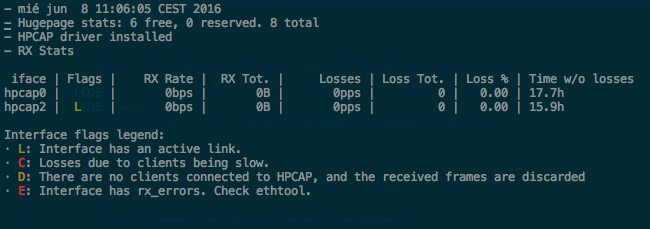
\includegraphics[width=0.8\textwidth]{figs/hpcap-status.png}
\caption{Script with the driver status. Each interface has statistics on the reception behaviour, and flags indicating its status.}
\label{fig:hpcap-status}
\end{figure}

The kernel log (\textit{/var/log/kernel.log} and/or \texttt{dmesg}, depending on the Linux distribution) will contain the messages from the driver that will show any error that may have happened.

HPCAP also provides interface monitors that log the bytes and frames received and lost\footnote{The monitor interval is configurable in the \textit{params.cfg} file}. These logs are accessible in the directory \textit{data/[year]-[week]}, with a file named for each interface. You can run \texttt{tail -f data/[year]-[week]/[interface]} to ensure that the monitor for that interface is running.

HPCAP integrates with the standard Linux networking tools, so commands like \texttt{ifconfig} or \texttt{ethtool} will be useful to check link status or the total losses of the interface.

\textbf{Note}: Both \textit{hpcap-status} and the monitor log files will only show received traffic when there's an application, such as \texttt{hpcapdd}, listening for data in the driver.


\section{Traffic capture: launching \texttt{hpcapdd}}
\label{sec:QuickCapture}

Once you have properly installed HPCAP on your system, you can use \texttt{hpcapdd} (or similar programs) to store the traffic from the network into your system.

\begin{enumerate}
\item Make sure you have enough space for traffic storage. It is recommended to use a different volume than the used for your operating system. You can check the space on each disk by executing \texttt{df -h}.

\item Launch the application (you will need superuser privileges). Assuming you've run already \texttt{make} and are in the \textit{HPCAP} directory, run \texttt{taskset -c 3 bin/release/hpcapdd 3 0 /storage }. In this case the application will fetch the traffic arriving to the queue $0$ on \texttt{hpcap3}. The core $3$ has been chosen in order to not interfere with the kernel-level capture thread and to avoid interception from different NICs (assuming a configuration as the one shown in~\ref{sec:example}).
\end{enumerate}

\section{Checking and reading captured traffic}
\label{sec:QuickStatus}

\begin{enumerate}
\item Check the counter files in the \texttt{data} subdirectory to ensure no losses have ocurred. You can use the script \textit{scripts/parse-hpcap-log}, that will summarize the log so you can tell easily the receive rate and whether losses ocurred during the capture. See \fref{sec:Monitoring} for more details on the monitoring facilities of HPCAP.

\item In your storage target directory, list the files that have already been written with \texttt{ls -lh /storage/*}. All of the generated files should have a size of 2 GB = 2147483648 bytes.

\item Convert one file from \texttt{raw} to \texttt{pcap} running \texttt{bin/release/raw2pcap  /storage/<dir>/<raw\_file>  <pcap\_file>}.

If the capture is being properly made, the program should end showing the message \texttt{Padding de XX bytes}, with XX being the amount bytes added at the end of the file for obaining a file size multiple of the filesystem's block size.

You can also use the application \texttt{bin/release/chechraw <storage\_dir>} to check that the RAW files are properly formed without converting anything. See \fref{sec:CaptureFiles} for more details.
\end{enumerate}

\section{When something is not working right}

Misconfigurations of the driver or unsual environments can cause the driver to perform badly or even crash. Some of these problems have easy workarounds:
\begin{itemize}
\item In some cases, the NIC may be failing to recognize certain VLAN encapsulations, and will throw frames where the unrecognized encapsulation plus the payload exceeds the card's MTU. The solution is to increase the MTU to accept those unrecognized frames: \texttt{ifconfig hpcapX mtu 1522} (or more bytes if necessary).
\item If the link has heavy traffic, HPCAP may fail to negotiate the speed and bring the link up, showing no Ethernet level link. The solution is to manually set the link speed with the comand \texttt{ethtool -s <iface> speed <link-speed> duplex full autoneg off}, where \texttt{link-speed} is the speed in Mbps (usually 10000).
\item Some applications and features may interfere and decrease HPCAP performance. Ensure the irqbalance service is deactivated and HyperThreading switched off.
\item Ensure that the driver's poll threads are running on the same NUMA node of the NIC card. See \fref{sec:NUMAArch} for details.
\end{itemize}

For other bugs and known errors, read \fref{sec:FAQ}. If the error persist, remember that the script \textit{scripts/diagnostics} will collect all necessary information from the system and pack it in a compressed file, so it can be sent to the developers for debugging.

\chapter{Installation}
\label{sec:Installation}

The basic installation procedure is explained in \fref{sec:QuickInstallation}. Here you can find more details on the requirements and installation modes.

\section{Requirements}

HPCAP is distributed as a source code, so you will need the build tools (\texttt{make} and \texttt{gcc}, mainly) and the Linux headers in order to compile the driver. Apart from this, you will also need some libraries and tools:

\begin{itemize}
\item \textbf{libpcap}: Both the library and the development headers. It's used for the samples that read or write to \textit{pcap} files.
\item \textbf{numactl}: Includes binaries, static library and the development headers. The binaries are used to detect NUMA architectures and configure the driver automatically. The library and headers are used to get the same information about NUMA architectures in some sample applications.
\end{itemize}

Apart from this, HPCAP may not build or run correctly with unsupported Linux kernel versions. HPCAP has been tested with the following versions: \supportedkernels.

Kernels other than the ones listed may introduce changes that can break the driver compilation, or make it fail at runtime.

\section{Installing the driver in the system}
\label{sec:SystemInstall}

The script \textit{install\_hpcap.bash} only loads the driver in the kernel, but does not actually install it. If you want to use HPCAP as a standard driver, you should run \texttt{sudo make install}. You can load the driver with \texttt{modprobe hpcap/hpcapvf} depending on which driver you want, or add it to the list of modules loaded at boot (\fileobj{/etc/modules}). Loading the module with modprobe or at boot time will automatically bring up the interfaces, but will not launch the monitors automatically.

In order to launch the monitors, you can run the command \texttt{launch-hpcap-monitors}.

The installation copies the driver binaries to the \textit{/lib/modules} folder, the samples and some scripts to \textit{/usr/bin} so they're accessible from anywhere, and the libraries and header files in \fileobj{/usr/lib} and \fileobj{/usr/include/hpcap} to build client applications.

\section{HPCAP folder contents}

The first step you must follow to use HPCAP in your system is obtain the HPCAP folder containing all the files related to the corresponding release. Inside this folder you will find the following subdirectories:

\begin{itemize}
\item \textit{bin}: Binary files, folder autogenerated by the \textit{Makefile}. Inside this folder there are two subfolders, one for each build configuration \textit{debug} and \textit{release}. You should normally use the binaries in the \textit{release} folder unless you want to debug a specific problem.
\item \textit{data}: The monitor log directory. Each HPCAP interface has a line for every containing the current timestamp, captured bytes, captured frames, missed bytes and missed frames.
\item \textit{doc}: Documentation files
\item \textit{driver}: Driver source code files.
\item \textit{include}: Common files (headers) for both driver and user level apps.
\item \textit{obj}: Intermediate build files, folder autogenerated by the \textit{Makefile}.
\item \textit{srclib}: Source files for the library used by user level level apps.
\item \textit{samples}: Several sample applications built for the HPCAP driver, including \textit{raw2pcap} and \textit{hpcapdd}.
\item \textit{install\_hpcap.bash}: Script that loads HPCAP in the system.
\item \textit{params.cfg}: Driver configuration.
\item \textit{scripts}: Scripts used to monitor and configure hpcap driver
\end{itemize}

\section{Testing the installation}

For testing whether the installation is correct or not, we can use the data folder. Here, the monitor programs keep a file for each capture interface, adding a new line every defined time (a second by default) with the captured traffic amount in that period. The \textit{hpcap-status} tool also shows a brief description of the captured traffic and HPCAP driver status.

It is important to notice that for these tools to work, there must be at least one consumer for the interface, like \texttt{hpcapdd}.

\chapter{Configuration}
\label{sec:Configuration}

As specified in the quick-start guide (\fref{sec:QuickStart}), the \textit{scripts/gen-hpcap-config} script can generate a basic configuration based on the information of the system and some sensible defaults that should be enough in most cases. However, when that configuration is not enough or when the performance obtained is not the expected one, you should know which are the configuration parameters of HPCAP and be able to tweak them to fit your needs.

\section{Configuration parameters}
\label{sec:Params}

All the scripts used for the installation and management of the HPCAP driver use of the information specified in the \fileobj{params.cfg} file that is located in the root level of the HPCAP folder, or in \textit{/etc/hpcap/} if the driver is installed in the system (see \fref{sec:Installation} for details). This file has to be properly modified so the HPCAP driver and dependant applications can properly run in your system.

Here you can find a list with parameters you must make sure to have properly configured before you run HPCAP:

\begin{itemize}
    \item \texttt{nif}: this parameter must contain the number of network interfaces available in your system (only the ones that would be managed by Intel's \texttt{ixgbe} driver). This number is ussually two times the number of PCI network cards plugged in your system (assuming you plug only 2-port cards), but this could vary if you use, for example, 1-port, 4-port network cards.

    \item \texttt{nrxq,ntxq}: number of RSS/Flow-Director queues that you want to use in your 10Gb/s network interfaces for both RX and TX purposes. The default value for this parameter is 1. It is not recommended to change this unless you know what changing this value implies.

    \item \texttt{consumers}: For the 40G version, controls the number of consumers for each queue. Consumer threads are allocated sequentally in the CPU space.

    \item \texttt{use\_vf}: Can be 1 or 0 depending on whether you want to install the virtual function driver or not.

    \item \texttt{ifs}: this is the list of interfaces that you want to be automatically woken up once the HPCAP driver has been installed. For each of those interfaces a monitoring script will be launched and will keep record of the received and lost packets and bytes inside the \texttt{data} subfolder, see \fref{sec:Monitoring} for details. See \fref{sec:InterfaceNaming} for more details on how the interfaces should be named.

    The interfaces in this options should be included in order and without gaps. That is, if you want to configure interfaces 1 and 3 in HPCAP mode, you should write all the interfaces until the fourth one: \texttt{ifs=''xgb0 hpcap1 xgb2 hpcap3''}. If you skip any interface, the installation scripts will not work.

    \item Interface-related parameters: those parameters must be configured for each one of the interfaces listed by the \texttt{ifs} parameter. All those parameters follow the format \texttt{<param\_name><itf\_index>} where \texttt{<itf\_index>} is the number identifying the index regardless the prefix to that number in the system's interface name (see \fref{sec:InterfaceNaming}). Those parameters are:
    \begin{itemize}
        \item \texttt{mode<itf\_index>}: this parameter changes the working mode of the interface between HPCAP mode (when the value is 2) and standard mode (if the value is 1). Note that an interface working in standard mode will not be able to fetch packets as interface in HPCAP mode would be able to, but the standard mode allows users to use for TX purposes (E.g.: launching a \texttt{scp} through this interface). An interface working in standard mode will no be able to be benefited byt the usage of the \texttt{detect-Pro10G} versions that can be found in the \texttt{samples} subfolder.

        A third mode is available: mode 3 will configure the interface with hugepage-backed buffers (see \fref{sec:Hugepages}). This mode is only used in the script, and internally mode 2 is used in the driver. The distinction is made only for automating the buffer mapping process with the script.

        \item \texttt{core<itf\_index>}: this parameter fixes the processor core of the machine that will poll the interface for new packets. As this poll process will use the 100\% of this CPU, affinity issues must be taken into account when executing more applications, such as detect-Pro10G. For further information see~\ref{sec:FAQ}.

        \item \texttt{vel<itf\_index>}: this parameter allows the user to force the link speed that will be negotiated for each interface. Allowed values are 1000 and 10000.

        \item \texttt{caplen<itf\_index>}: this parameter sets the maximum amount of bytes that the driver will fetch from the NIC for each incoming packet.

        \item \texttt{pages<itf\_index>}: amount of kernel pages to be assigned to this interface's kernel-level buffer. The installation script will check the amount of pages to be used and make sure the sum of the pages used by all interfaces in HPCAP mode is the total. If this condition is not met, the installation script will issue an error message with useful information for changing this configuration.

        \item \texttt{hugesize<itf\_index>}: buffer size for interfaces in mode 3. Will be aligned to hugepage size at runtime. Can be a human-readable size, such as 2GB or 4096MB.

%       \item \texttt{dup<itf\_index>}: this parameter enables or disable duplicate removal for the corresponding interface. This parameter will only take effect is the interface is configured to work in HPCAP mode..

    \end{itemize}

    \item \texttt{monitor\_enabled}: Can be 1 or 0. If 1 (enabled), the \textit{install\_hpcap.bash} script will launch the monitors for the HPCAP interfaces.

    \item \texttt{monitor\_basedir}: Where to save the monitoring logs when the driver is installed in the system. The logs will be saved in \textit{HPCAP/data} if the driver is not installed but is running from the source folder.

    \item \texttt{monitor\_interval}: Sampling interval, in seconds, for the interface monitors.

    \item \texttt{monitor\_core}: Core in which the monitors will run. Useful when the scripts interfer with the kernel or capture threads.
\end{itemize}

\textbf{Warning:} changing any of the above mentioned parameters will take no effect until the driver is re-installed.

Once all the configuration parameters have been properly set, the execution of the script \texttt{install\_hpcap.bash} will take charge of all the installation steps that need to be made in order to install the HPCAP driver.

\subsection{Hot swapping parameters}
\label{sec:Params:HotSwapping}

Some HPCAP parameters can be changed while it is running. It can be done using the script \texttt{change-config.sh} under the directory \texttt{scripts} with several parameters.

The currently implemented functionality includes:
\begin{itemize}
    \item \texttt{+dups/-dups}: Enables (+) or disables (-) duplicate removal.
\end{itemize}

\section{Interface naming and numbering}
\label{sec:InterfaceNaming}

This version of the driver allows choosing whether each interface is to work in HPCAP or standard (traditional, \texttt{ixgbe}-alike) modes. Consequently, a decision regarding the naming policy for those interfaces was made.

The target of this policy was always being able to identify each of the interfaces of our system regardless the mode it is working on (so you will be able to know which \texttt{<param\_name><itf\_index>} of the \texttt{params.cfg} file maps to each interface). This leaded to each interface being named as \texttt{<mode\_identifier><interface\_index>}, where:
\begin{itemize}
    \item \texttt{<mode\_identifier>}: can be \texttt{hpcap} when the interface is working in the HPCAP mode, or \texttt{xgb} if the interface works in standard mode.

    \item \texttt{<interface\_index>}: this number will always identify the same interface regardless its working mode. For example, if the first interface found in the system is told to work in standard mode and second interface in the HPCAP mode, you will see that your system has the \texttt{xgb0} and \texttt{hpcap1} interfaces. If you revert the working mode for such interfaces you will then find interfaces named \texttt{hpcap0} and \texttt{xgb1}.
\end{itemize}

The number assigned to each interface is fixed across reboots, as it is based on the order assigned by the PCI bus and function index of each port.

\section{Multicore architectures}
\label{sec:NUMAArch}

Given the performance requirements of HPCAP, a careful configuration in multicore systems is needed. HPCAP launches a polling thread for each interface. These threads should be placed in the same NUMA node as the physical card for optimal performance, using the \texttt{core} parameter of each interface (see \fref{sec:Params}).

In order to get the NUMA node of the NIC, you can either use \sysobj{lstopo} from the \textit{hwloc} package or read the file \textit{sys/bus/pci/devices/0000:[PCI ID]/numa\_node}, where \textit{PCI ID} is the ID of the NIC that you can extract from the output of \sysobj{lspci}. A sample for both options is provided below.

\begin{lstlisting}[language=C, caption={Obtaining NUMA information.}, label={lst:NUMA}]
$ lstopo
Machine (128GB)
  NUMANode L#0 (P#0 64GB)
    ...
    HostBridge L#0
      PCIBridge
        PCI 8086:1521
          Net L#0 "eth0"
        PCI 8086:1521
          Net L#1 "eth2"
      PCIBridge
        PCI 8086:10fb
          Net L#2 "hpcap0" <-- NIC in node 0
        PCI 8086:10fb
          Net L#3 "xgb1"
    ...

$ lspci
...
05:00.0 Ethernet controller: Intel Corporation 82599EB 10-Gigabit SFI/SFP+ Network Connection (rev 01)
05:00.1 Ethernet controller: Intel Corporation 82599EB 10-Gigabit SFI/SFP+ Network Connection (rev 01)
...

$ cat /sys/bus/pci/devices/0000\:05\:00.0/numa_node
1
$ cat /sys/bus/pci/devices/0000\:05\:00.1/numa_node
1
\end{lstlisting}

The capture applications should be placed in cores different than the used for the HPCAP threads. Based on \cite{m3omon}, it seems that the optimal configuration is to put the capture applications in a different NUMA node from the HPCAP cores. However, this depends on the specific system you are using, so you should test with different configurations if you are not getting enough performance (that is, HPCAP is losing frames).

You should also ensure that the kernel does not use the cores assigned to the HPCAP threads and capture applications to schedule other processes. Knowing the list of cores to be assigned, you must isolate them using the boot parameters of the system. Depending on the distribution we are using:

\begin{itemize}
    \item \textbf{OpenSuse:} you have to edit the \texttt{/boot/grub/menu.lst} file and add into the boot desired command line the following: \texttt{isolcpus=0,1,2,..,k} (with \texttt{0,1,2,..,k} are the CPUs to be isolated). The next time you boot your system your changes will have taken effect.

    \item \textbf{Ubuntu/Debian:} you have to edit the \texttt{/boot/grub/menu.lst} file, and in the \texttt{GRUB\_CMDLINE\_LINUX\_ DEFAULT} parameter add the following: \texttt{isolcpus=0,1,2,..,k}. Then, execute \texttt{update-grub} and the next time you boot your system your changes will have taken effect.

\end{itemize}

\section{Using hugepages}
\label{sec:Hugepages}

The HPCAP driver can use hugepage-backed buffers to increase the buffer size and access speed. The install script manages this automatically when interfaces are set in mode 3 (see section \ref{sec:Params}). However, it expects the \textit{hugetlbfs} to be mounted in \textit{/mnt/hugetlb}. The script \textit{hugepages\_mount} can be used to mount this filesystem automatically.

In order to use hugepages, your system must be configured properly at boot time. That means that you should add the corresponding parameters to the \textit{linux} command in your \textit{grub.cfg} file. These parameters are \textit{default\_hugepagesz, hugepagesz} and \textit{hugepages}, as documented in the kernel documentation. For example, the parameters \texttt{default\_hugepagesz=1G hugepagesz=1G hugepages=8} would enable hugepages of 1 GB, and then would allocate 8 hugepages of 1GB at boot time. In the end, your \textit{linux} boot command could look like this:

\texttt{linux /boot/vmlinuz-3.8.0-29-generic root=UUID=b2be13dc-7a60-4928-b61a-cc3ec95044a0 iommu=pt intel\_iommu=on isolcpus=0,1,2,3,4,5 ro default\_hugepagesz=1G hugepagesz=1G hugepages=8}

If you want to make the hugepage configuration persistent even when GRUB is updated, you should add the parameters to the \textit{/etc/default/grub} file.

You can check if the hugepages were assigned correctly by running \texttt{grep ``Huge'' /proc/meminfo}. More information regarding the inner workings of hugepages can be found in the developer guide of HPCAP.

In order to use hugepages, you have to set the interface in mode 3 and assign it a size with the \texttt{hugesizeX} parameter (see \fref{sec:Params} for details on the configuration options).

\subsection{Memory limits}
\label{sec:Hugepages:Memlimits}

Linux systems usually have a limitation of the amount of memory that can be allocated by a single process. This can cause errors when trying to allocate big buffers backed by hugepages. The first limit to check should be the user limits (\textit{ulimit -a}) enforced by the system.

If the memory is unlimited for the user, then the kernel could be limiting the amount of shared memory and shared memory segments. They can be checked by running the commands \texttt{sysctl kernel.shmmax} and \texttt{sysctl kernel.shmmni}. The most important is \textit{shmmax} as it limits the amount of shared memory of a process, and has a default value of 4 GB (4294967295 bytes). These limits can be changed by running the commands:
\begin{verbatim}
sudo sysctl -w kernel.shmmax=[newvalue]
sudo sysctl -w kernel.shmmni=[newvalue]
\end{verbatim}

For the memory segments limits, usually doubling the default value of 4096 is enough.

\chapter{Usage}
\label{sec:DriverUsage}

\section{Traffic capture}
\label{sec:Capture}

The capture process can be done as explained in \fref{sec:QuickCapture} or using other applications that call the HPCAP library. HPCAP provides two simple applications that capture and store traffic.

\subsection{hpcapdd}
\label{sec:hpcapdd}

\texttt{hpcapdd} is a sample program that maps HPCAP's kernel packet buffer for a certain interface and write its contents into the desired destination directory.
Note that, in order to obtain maximum performance, the data access is made in a byte-block basis. This byte-block access policy has consequences regarding its usability, as it must be assured that the application starts running in a correct state.
\texttt{hpcapdd} will generate data files following the RAW format (see~\fref{sec:raw}).

\texttt{hpcapdd} has been programmed so it performs an orderly close when receiving a \texttt{SIGINT} signal, so it must be ended with \texttt{kill -s SIGINT ...} or \texttt{killall -s SIGINT ...}.

\subsection{hpcapdd\_p}
\label{sec:hpcapddp}

\texttt{hpcapdd\_p} is a sample program that maps HPCAP's kernel packet buffer for a certain interface and write its contents into the desired destination directory.
Note that \texttt{hpcapdd\_p} accesses the data in a per-packet rather than in a byte-block basis. This decreases the write throughput performance but may result of interest as it has some interesting usability effects.
\texttt{hpcapdd\_p} will generate data files following the RAW format (see~\ref{sec:raw}).

As with \texttt{hpcapdd}, \texttt{hpcapdd\_p} has been programmed so it performs an orderly close when receiving a \texttt{SIGINT} signal, so it must be ended with \texttt{kill -s SIGINT ...} or \texttt{killall -s SIGINT ...}.

\subsection{Reading the capture files}
\label{sec:CaptureFiles}

As explained in \fref{sec:raw}, HPCAP generates RAW files. These can be converted to PCAP using the program \fileobj{raw2pcap}\footnote{Found with the rest of the applications in the \textit{bin/release} folder after compilation.}.

To check the integrity of the captured files, the program \fileobj{checkraw} can also be used: it receives as argument the directory where all the files are stored, and then goes on checking all of the frames and that they are saved in the correct format. Optionally, the program can receive a minimum timestamp as a second argument. If it encounters file with an older timestamp, it will ignore them.

\section{Interface monitoring}
\label{sec:Monitoring}

HPCAP provides monitoring scripts that log the performance of the capture for each interface. The data generated by those monitoring scripts can be found in the \texttt{data} subfolder or, when the driver is installed in the system, in the directory specified in the \textit{params.cfg} file. In order to avoid the generation of single huge files, the data is stored in subfolders whose names follow the format \textit{[year]-[week number of year]}.

Inside each of those \textit{[year]-[week number of year]} subfolders, you will find a file for each of the active interface plus a file with CPU and memory consumption related information. The fields appearing in each of the \textit{hpcapX} files are:
\begin{verbatim}
    <timestamp> <RX-bps> <RX-pps> <lost-bps-estimate> <lost-pps>
\end{verbatim}

Additionally, in the log directory you will find files named \textit{iface-monitor.log} and \textit{iface-monitor.pid} for each interface monitored. These store the output of the monitor (useful to see if any errors have been happening) and the PID of the process, that can be used to terminate it automatically.

To launch and stop the monitors, you can use the \fileobj{launch-hpcap-monitors} and \fileobj{stop-hpcap-monitors} in the \textit{scripts} folder or in your PATH if you have installed the driver.

For easy reading of these logs, the script \textit{scripts/hpcap-status} is provided: it will continously print in an easily readable form the status of the drivers: link state, hugepage allocation stats, reception rate and loss stats.

\subsection{Parsing the monitor log}

The script \fileobj{parse\_hpcap\_log} has been created to help in the analysis of the HPCAP monitor logs. This script receives two arguments: the log file itself and, optionally, the monitoring interval in seconds (by default it's set to 1).

It then reads the log file, extracting the relevant entries (it does so by stripping entries with zero frames received and lost from the beginning and the end of the file) and parsing relevant details, such as test begin/end date, average, maximum and minimum transfer speeds and lost frames. It also outputs a simple timeline made by grouping the entries depending on whether they had losses or not. It will print something similar to this:

\begin{lstlisting}
At Wed Sep 17 21:53:18 CEST 2014 (ts 1410983598, elapsed 0 secs) all ok (1 secs). Received 755952 frames, 4256.85 Mbits, 4.157 Gbps.
At Wed Sep 17 21:53:20 CEST 2014 (ts 1410983600, elapsed 1 secs) losses (5 secs). Lost 11083 frames. Received 8468847 frames, 48153.52 Mbits, 9.404 Gbps.
At Wed Sep 17 21:53:25 CEST 2014 (ts 1410983605, elapsed 6 secs) all ok (1 secs). Received 1702646 frames, 9675.18 Mbits, 9.448 Gbps.
At Wed Sep 17 21:53:26 CEST 2014 (ts 1410983606, elapsed 7 secs) losses (4 secs). Lost 16807 frames. Received 6617632 frames, 37389.83 Mbits, 9.128 Gbps.
At Wed Sep 17 21:53:30 CEST 2014 (ts 1410983610, elapsed 11 secs) all ok (1 secs). Received 1690432 frames, 9679.26 Mbits, 9.452 Gbps.
\end{lstlisting}

This allows to see easily in which intervals the driver performed with zero losses and at which rates, and also to see where and how many frames were lost, and during how much time.

Finally, if the system can output \textit{gnuplot} graphs, it will generate a plot of the monitored speed and frame losses.

\subsection{Monitoring CPU usage}

Apart from the monitring scripts, the script \fileobj{monitorCPUs.bash} can monitor the CPU usage of the system and related applications. The log, \textit{cpus}, is written in the same directory as the \textit{hpcapX} with the following fields:

\begin{verbatim}
    <timestamp> <\%-of-used-CPU(one for each CPU)> <total-memory> <used-memory> <free-memory >
        <cached-memory> <detect-pro-memory-consumption(one for each instance, 0 if none) >
\end{verbatim}

\section{Waking up an interface in standard mode}
\label{subs:standard}

If a interface configured to work in standard mode wants to be configured, the \texttt{wake\_standard\_iface.bash} script is provided. Its usage is the following:

$\;\;$ \texttt{./wake\_standard\_iface.bash <iface> <ip addr> <netmask> <core> [<speed, default 10000>]}

Where:
\begin{itemize}
    \item \texttt{iface} is the interface you want to wake up. As this is thought for interfaces working in standard mode, the interface should be some \texttt{xgbN}.

    \item \texttt{<ip addr> <netmask>} are the parameters needed to assign an IP address and a network mask for this interface.

    \item \texttt{core} is the processor where all the interrupts regarding this will be sent, so we can make sure that such interrupts do not affect the capture performance of an HPCAP interface.
    \item \texttt{speed} is an optional parameter that allows you to force the link speed of this interface. Its values can be 1000 or 10000.

\end{itemize}

\section{Collecting diagnostic data}
\label{sec:DiagnosticData}

If a failure occurs, the file \fileobj{scripts/diagnostics} can be used to collect information to help the developer of the driver to diagnose the issue. See the developer guide for details on the information collected.

\chapter{API}

This section is intended for developers of programs that interact with HPCAP, reading from its buffer. There are two ways to read from the HPCAP buffer, one easier and quick, and the other one more complex but with more possibilities.

\section{Step 0: installing the libraries}

Regardless of the used library, it is recommended to install the libraries to the system to avoid problems with relative routes and similar issues. If you are developing your code in the same machine on which HPCAP will be running and capturing traffic, you can just install the driver with \texttt{sudo make install}. This will install the driver (see \fref{sec:Installation}) and copy the libraries and headers to the respective system locations \textit{/usr/lib} and \textit{/usr/include}. In this way, you will be able to use the HPCAP libraries just as any other system library.

However, you might be developing your code in one machine different from the one where the driver is installed. For this situation, you can install only the libraries and headers with \texttt{sudo make install-libs}: you will be able to compile your program and have autocompletion if your editor provides it, but without installing unnecessary drivers and configurations to your machine.

\section{libmgmon: Easy access to HPCAP packets}

The mgmon library gives easy access to the HPCAP buffer, either packet-by-packet or grouping by flows, using a similar call that what . It is best shown with an example:

\begin{minted}[breaklines=true]{c}
#include <stdlib.h>
#include <stdio.h>
#include <libmgmon.h>

/**
 * A structure for easy parsing of Ethernet frames
 * Source: http://lxr.free-electrons.com/source/include/uapi/linux/if_ether.h#L139
 */
struct ethhdr {
    unsigned char   h_dest[ETH_ALEN];       /* destination eth addr */
    unsigned char   h_source[ETH_ALEN];     /* source ether addr    */
    __be16          h_proto;                /* packet type ID field */
} __attribute__((packed));

void handle_packet(uint8_t* payload, struct pcap_pkthdr* header, void* arg) {
    struct my_struct data = (struct my_struct*) arg; // Use the arg pointer to store any data you need to pass down to the handler

    // header->ts contains the timestamp of the packet (struct timeval)
    // header->caplen contains the bytes that were captured for this packet. This is the length of the payload argument.
    // header->len is the length of the packet as was seen on capture. Note that it may not be the same as caplen.

    if (header->caplen < size(struct ethhdr)) {
        // Important: always check caplen (not len) to ensure that you have enough data.
        printf("Not enough length to parse Ethernet\n");
        return;
    }

    // Example: parse ethernet header.
    struct ethhdr* eth = (struct ethhdr*) payload;

    // ...
}

int main(int argc, char** argv) {
    struct my_struct data;

    // ...
    int cpu = 1; // Choose the CPU carefully (see section on multicore archs) for best performance
    int iface = 0; // The interface to listen on (e.g., hpcap0 is iface 0)
    int qindex = 0; // Queue is usually 0.

    // Start the listening loop
    mgmon_packet_online_loop(cpu, iface, qindex, handle_packet, &data);
}
\end{minted}

You can stop the receive loop by passing a SIGINT (Ctrl-C) signal to the process.

\section{libhpcap: Raw access to HPCAP}

The libhpcap library provides raw access to the HPCAP structures, and is the base for the other libraries. You should probably not use this library unless you know why you want it and you how HPCAP works and interacts with your program.

Although all the functions are documented in \fileobj{hpcap.h}, you may want to generate automatic documentation with Doxygen. To do this, run \texttt{make doxydoc} and open the file \textit{doc/html/index.html} with your favourite browser.

\section{Notes for the HPCAP API user}

When developing for the HPCAP API, you must have some details in mind:

\begin{itemize}
\item HPCAP follows the slowest listener. If your program is too slow, the buffer will fill up and HPCAP will start dropping packets for all applications connected to HPCAP. Keep this in mind when deploying multiple applications reading from the same interface: low performance spikes or hangs in one program will cause loss of packets on \textit{all} applications. You can see if this is happening by reading the output of \textit{hpcap-status} (\fref{sec:QuickStatus}).
\item Core assignment is important. Read the \fref{sec:NUMAArch} on multicore architectures to understand how to assign HPCAP and application cores for maximum performance.
\end{itemize}

\chapter{Frequently asked questions (or maybe not so frequent)}
\label{sec:FAQ}

\paragraph{Which Linux kernel versions does HPCAP support?}
    HPCAP has been written for working under diverse Linux kernel/distribution combinations. Specifically, it has been tested for the following versions:
    \begin{itemize}
        \item \textbf{OpenSuse:}  2.6.32 .
        \item \textbf{Ubuntu/Debian:} 2.6.32, 3.2.0, 3.11.0, 3.13.0, 3.15.0, 3.19.0.
        \item \textbf{Fedora:} 3.5.3, 3.14.7 .
    \end{itemize}

\paragraph{Should I always use all the available interfaces in \texttt{hpcap} mode?} \par
    No. The reason for this is that the total amount of memory that this driver can use as internal buffer is 1GB, and this amount is divided between the \texttt{hpcap} interfaces present in your system. Thus, if you are not going to capture packets from one interface configure it to work in standard mode and you will have bigger buffers for your capturing interfaces. The amount of memory assigned to each interface out of this 1GB is configured via the \texttt{pages} parameter (see \fref{sec:Params}).

\paragraph{Can I use more than one RX queue?}
    If you are going to use Detect-Pro the answer is no. The current version of Detect-Pro support packet capture for just one RX queue. Otherwise you can use more than one RX queue by changing \texttt{nrxq} parameter in the \texttt{params.cfg} file. Notice that if you use more than one queue per interface you will need to instantiate several packet-consuming applications (at least one per queue) in order to fetch all the data).

\paragraph{Can I simultaneously capture data from an interface with \texttt{dd} and \texttt{hpcapdd}?}
    Yes. In fact, you can use any amount of \texttt{dd} or \texttt{hpcapdd} instances over the same pair (interface,queue). The limit on the amount of simultaneous applications fetching data from the same pair (interface,queue) is defined in the \texttt{include/hpcap.h} file with the \texttt{MAX\_LISTENERS} constant. Note that a change in this value will take no effect if the driver is not recompiled and re-installed in your system.

\paragraph{I am not obtaining the expected network capture performance, what is happening}
    The most probable cause is a misconfiguration of the core assignments. See \fref{sec:NUMAArch} for details, but you should make sure that you have properly set the processor affinity for your storage programs (\texttt{dd}, \texttt{hpcapdd}) via the \texttt{taskset} command) and that the assigned processor is not used by any kernel capture thread.

    You can also check the script \textit{hpcap-status} or the counter \texttt{rx\_hpcap\_client\_lost\_frames} in \textit{ethtool}\footnote{Run \texttt{ethtool -S hpcapX} to see the counters of the interface.} to check if the losses are due to slow clients or if it's the driver the one losing them.

\paragraph{I see no traffic from the counters that appear on the \texttt{data/<year>-<week>} files}
    This is normal behaviour. Until there is at least one application listening, the kernel driver will not fetch packets and thus all the counters will be zero. Nevertheless, if the traffic intensity is very high, it is possible that the lost counter will be incremented but the amount is not to be trusted. This is a known issue that has not been solved yet.


\paragraph{Is it possible to change the size of the RAW files generated by \texttt{hpcapdd} or Detect-Pro?}
    Yes, you can. Remember the default file size is 2GB, which was chosen as a tradeoff between  write performance ans data accesibility.
    However, if this file size does not fit your requirements you can change it (altough it is not reccommended due to the delicate operations involved) by editing the following parameter in the \texttt{HPCAP/include/hpcap.h} file:

        \begin{center}
            \texttt{\#define HPCAP\_BS ( 1048576ul )}\\
            \texttt{\#define HPCAP\_COUNT ( 2048ul )}\\
            \texttt{\#define HPCAP\_FILESIZE (HPCAP\_BS*HPCAP\_COUNT)}\\
        \end{center}

    Changing the block size (\texttt{HPCAP\_BS} parameter) is discouraged, so the right way of changing the generated files' size is changing the \texttt{HPCAP\_COUNT} parameter.

    \textbf{Important:} after changing these parameters (or anyone in the \texttt{hpcap.h} header file, it is required to re-compile the driver and any of the sample applications based on HPCAP used.

\paragraph{How can I know which driver version am I running?}
    The build system automatically generates the build information and includes it in the driver file. To get it, run \texttt{modinfo driver -F version}, where \texttt{driver} is either the path to the driver \textit{.ko} file or the name of the driver (\textit{hpcap} or \textit{hpcapvf}) if it has been installed to the system. The output will be something similar to this:

    \vspace{3pt}
    \termcommand{modinfo hpcap -F version \\
    HPCAP v4.1.0 built Sat Aug 22 16:18:05 CEST 2015 IXGBE 3.7.17-NAPI}
    \vspace{3pt}

    The \textit{v4.1.0} indicates the version of HPCAP. It's automatically generated by the build script based on the output of \textit{git describe}, so if you are not using a stable release you can see something along the lines of \textit{v4.1.0-7-g1237abc}: it shows that the driver has beeen build from the commit with abbreviated hash \textit{1237abc}, 7 commits after the 4.1.0 version. It

    The last part of the version string refers to the base IXGBE version that was used to create the HPCAP driver.

\paragraph{The driver installation fails with ``Cannot allocate memory''}
    Check the kernel log, further instructions and details should be there. For example, it could be related to the configuration of the pages for each adapter: you should check that there are no more pages assigned that pages are available. The available page count depends on the \codeobj{HPCAP\_BUF\_SIZE} macro and is printed in the kernel log when the page configuration is incorrect.

\paragraph{The driver installation fails with ``Unknown symbol in module''}
    Check the kernel log. If it says something similar to \textit{hpcap: Unknown symbol vxlan\_get\_rx\_port (err 0)} try running \texttt{modprobe vxlan} before installing.

% -*- root: ../HPCAP_DevGuide.tex -*-
\section{Bugs, system errors and known issues}
\label{sec:bugs}

This section shows the bugs that have been found during the development and use of the driver, hoping that it gives the reader some ideas when the driver and/or the kernel have turned crazy and decided not to work.

\subsection{Driver/system corruption after system crash}
\label{sec:bugs:drivercorrupt}

\begin{bugdata}
\bugfixed[06b9ec8: insmod: Blacklist hpcap and ixgbe to avoid loading them at unusual times
]
\versions{4.2.0, 4.2.1}
\end{bugdata}

During the testing of HPCAP 4.2.1, the system crashed because of unknown issues while HPCAP was receiving traffic. The driver was installed to the system. After a reboot, something was corrupted: both \textit{ixgbe} and \textit{hpcap} were loaded at boot (even though none of them was configured to do so) and could not be removed. Trying to install the module again resulted in either errors or \textit{modprobe/insmod} hanging.

It seems that, after a crash, the Linux kernel tries to reload the modules in some weird fashion, reloading both \textit{ixgbe} and \textit{hpcap} and causing some weird conflicts, including errors in the Intel Direct Cache Access subsystem (in some instances, the driver crashed on install with the stack trace pointing to \texttt{dca\_register\_notify}).

% Comment to facilitate searching: dca_register_notify

The fix was to blacklist both drivers in the \textit{modprobe} configuration that was already being generated on install. When the error happened, the system could be restored running \texttt{depmod -a \&\& update-initramfs -u} with \textit{root} permissions, or reinstalling the kernel.

\subsection{Segmentation fault on client applications}

\begin{bugdata}
\bugfixed[9f21f1f: Fix concurrency issue when adding listeners]
\versions{4.1.0 and previous}
\end{bugdata}

Sometimes, when multiple clients open the same HPCAP handle at the same time (for example, \sysobj{monitor\_flujos} opens two handles on the same file), a race condition may occur and the listener identifications will not be registered correctly. This causes messages in the kernel log warning about some ``listener not found'' and possibly a segmentation fault when issuing \texttt{ioctl} calls. The solution was to properly protect critical sections of the code that can be read and written concurrently.

\subsection{modprobe/insmod: Cannot allocate memory}

\begin{bugdata}
\bugnotfixed
\versions{All}
\end{bugdata}

There are several possible causes. If the error is raised by the HPCAP driver, you should see a line in the kernel log explaining what happened and how to correct the error\footnote{If the message appears but does not tell how to fix the error or does not explain what's happening, tell the maintainer to change that error message.}.

However, if the kernel log doesn't show any message from \textit{hpcap}, it may be an issue with available memory in the kernel. The Linux kernel has a certain memory space assigned to load modules\footnote{See \href{https://www.kernel.org/doc/Documentation/x86/x86_64/mm.txt}{the kernel documentation about the matter}.}, usually about 1.5GB. It's more than enough for regular uses of modules, but not in the case of HPCAP. HPCAP allocates a static buffer of 1GB that will be shared between the different queues. This buffer is placed on that module mapping space\footnote{It may be possible that I'm wrong here about this.} so, if several modules have already reserved more than 500 MB, the kernel may refuse to load our module.

The workaround for this is to reduce the buffer size (modify the macro \codeobj{HPCAP\_BUF\_SIZE} in the \fileobj{include/hpcap.h} file) and, if necessary, to use hugepages (see \fref{sec:Hugepages}) to get buffers of the necessary size. I haven't found any way to see the memory usage of each driver nor how to see how much of that module mapping space is already allocated.

\subsection{Interfaces renamed automatically by udev}
\label{sec:bugs:IfaceRenaming}

\begin{bugdata}
\bugfixed[r715: insmod: workaround for udev renaming rules, r807]
\versions{4.2.2 and previous}
\end{bugdata}

In some systems, udev has some ``smart'' renaming rules \href{http://www.freedesktop.org/wiki/Software/systemd/PredictableNetworkInterfaceNames/}{that theoretically gives a predictable naming to the network interfaces}. That interferes heavily with HPCAP. The workaround consists in a small check in the \codeobj{interface\_up\_hpcap} bash function, that will check in the kernel log for \textit{udev} renamings and will undo them.

An extra problem in some CentOS installations was that \textit{udev} did not even print in the kernel log these renames. This required an extra fix (revision 807 in \textit{mellanox} branch, merged into trunk in rev. 838), that consisted of a naming check (the actual function is called \codeobj{hpcap\_check\_naming}) that is called before launching the poll threads. This functions compares the current name of the interface to the expected one (\textit{hpcapX}, where \textit{X} is the adapter index): if they are different, it prints a message to the kernel log that will be picked up by the installation script so it can rename the interfaces.

\subsection{Corrupted capture files}
\label{sec:bugs:CorruptedCapture}

\begin{bugdata}
\bugfixed[r842, r869]
\versions{4.2.3 and previous}
\end{bugdata}

A bug was discovered where the captures were being corrupted if another program had been listening previously. For example, if a first instance of \textit{hpcapdd} was launched and then closed, the resulting capture files were all correct. However, if a second instance was launched without reinstalling the drivers, all capture files would be corrupted.

The actual issue had to to with how the clients (listeners) acquire their reading offsets. A first listener would start reading from offset 0, transferring blocks of a fixed size. When the client closed, HPCAP saved the last reading offset, which would not necessarily point to the beginning of a frame.

Thus, when another new client tried to read from the HPCAP buffer, its reading offset was the last reading offset of the other client. This new client would begin saving the capture at the middle of a frame, so applications such as \textit{raw2pcap}, expecting to read first a correct packet header, would crash and/or output completely wrong results.

A first solution was to assign as read offset the last writing offset of the HPCAP producer. New frames are written starting from that offset, so new listeners would start reading frames with the correct headers. However, this caused another extra problem: misaligned access to the buffer that could hurt performance. A fix for this issue is simply resetting the read/write offsets when there are no listeners: if there are no client applications, HPCAP will forget the last read/write offsets and will start writing frames from offset 0, thus avoiding misaligned access for new clients.

A secondary bug appeared later, introduced by the first fix (r842): in some cases the global write offset would be advanced before the read offset of a new listener was configured. In these cases, the read offset would again be greater than 0 and would cause errors when writing the captures. This bug was fized in r869 by setting the read/write offsets in the intialization of the listener.

\subsection{Connection failure / segfault on xgb interfaces}

\begin{bugdata}
\bugfixed[r826: ixgbe: Fix bug with ixgbe interfaces where next\_to\_use wasn't being updated and caused errors]
\versions{4.2.3. Possibly previous versions, not checked}
\end{bugdata}

Interfaces configured in the \textit{xgb} mode were failing and/or crashing the system completely when they received data.

The cause was that the \texttt{rx\_ring->next\_to\_use} pointer was not updated correctly. It should be updated in \codeobj{ixgbe\_release\_rx\_desc} to have the same value as the ring's tail pointer of the NIC, but the corresponding line was missing. This caused incoherencies between the ring status in software and in hardware, which in turn caused missing frames (thus the failing connections) and even crashes when the software tried to access to unallocated descriptors.

\subsection{Connection reset after TX hang}

\begin{bugdata}
\bugfixed[r875, r876: ixgbe: Disable transmission and forced resets on TX hangs]
\versions{4.2.3 and previous}
\end{bugdata}

If an application in the system tried to send frames through interfaces configured in HPCAP mode, it could trigger a reset in the interface that would lead to corrupted captures.

The bug was that the \textit{ixgbe} driver would store the packets to send in a queue which was not flushed. Then, a watchdog (either in the driver or in the kernel) would notice\footnote{The exact message was \textit{initiating reset due to lost link with pending Tx work}.} and reset the adapter. This would in turn reset the poll thread and corrupt the capture.

The solution was to discard frames to transmit in HPCAP adapters, and to disable the code that resets the adapter when using HPCAP work modes.

\subsection{Loss of all frames}
\label{sec:bugs:AllFramesLost}

\begin{bugdata}
\bugfixed[r963: hpcap: Fix bug where the driver was losing all frames]
\end{bugdata}

A misterious bug where at random times caused the driver to lose all frames. The cause was the padding check. When receiving a packet, if the space left in the capture file was exactly 2 RAW headers plus the incoming packet size, no padding would be written. The space left for the next frame was exactly the size of the RAW header, so the padlen, calculated as the remaining space in file \textit{minus the size of a RAW header} would be zero and no padding would be inserted. The file size would be also incremented, surpassing the value of \texttt{HPCAP\_FILESIZE} and either corrupting the memory space when writing with erroneous lengths or avoiding the reception of any packets as the driver would not have space to insert the padding with that size.

\subsection{IOCK and MNG\_VETO bit enabled - capture thread stops}

\begin{bugdata}
\bugnotfixed
\versions{pre-5.0.0, at least}
\end{bugdata}

In a certain installation, the driver would stop capturing after the system received a non-maskable interrupt about an IOCK error. There is not much documentation about this error, but it seems to be related with the hardware.

The kernel log also showed a message from the base \textit{ixgbe} driver about a \texttt{MNG\_VETO}\index{MNG\_VETO} bit enabled. Reading the NIC datasheet \cite{825992010}, it seems to be a bit set up by the hardware when it is in low-power state that forbids link changes, so downed links would not be restored.

As of 27/4/2016, this bug seems to be caused by the hardware.

\subsection{Concurrent listeners leads to losses and/or data corruption}

\begin{bugdata}
\bugfixed[r959, r955]
\versions{4.2.3 and previous}
\end{bugdata}

Several related errors happened when there was more than one client listening for data in a HPCAP interface. For example, if a listener connected first but did not read anything, a second listener would receive an advanced read offset (the last write from the polling thread). So, even when the two listeners could start reading data from the buffer at the same time they would see different data. This was fixed in revision 959.

Another problem happened when two listeners connected to the driver and then the first one disconnected. The next listener to connect would receive handle ID 2, which was already being used. Data loss and/or corruption of the structures would then occur. This was fixed in revision 955.

\subsection{Copies from/to user space can fail}

\begin{bugdata}
\bugfixed[r956: hpcap: Fix copies from/to the user memory]
\versions{4.2.3 and previous}
\end{bugdata}

In the \texttt{ioctl} calls, the copies to and from user space memory were not being done with \texttt{copy\_to/from\_user} and, in strange instances where that memory was invalid, that could cause a segfault within the driver. With the fix, no invalid acceses are done and the correct error message is returned to the caller application.

\subsection{Corrupted capture files after restarting a client}

\begin{bugdata}
\bugfixed[r893: hpcap: Reset written buffer size when there're no listeners]
\versions{4.2.3 and previous}
\end{bugdata}

Related to bug \ref{sec:bugs:CorruptedCapture}, when restarting a listener, the captures would be subtly corrupted as the driver would not place the padding at the end of the file but in the middle instead. This happened because the filesize counter was not being reset if there were no listeners.

\subsection{Problems when using buffers greater than 2GB}

\begin{bugdata}
\bugfixed[r990: hpcap: Fix several problems with buffers greater than 2G]
\versions{4.2.X}
\end{bugdata}

When using hugepage-backed buffers with a size greater than 2GB, several variables would overflow and cause segfaults and memory errors.

There is a secondary problem: when allocating buffers of size 4GB, the function \codeobj{vm\_map\_ram} used in the hugepage code will segfault due to a bug in the Linux kernel code. See \href{http://marc.info/?l=linux-mm&m=146114962421719&w=2}{the linux-mm mailing list} for more information. The patch was included in kernel version 4.7.

\subsection{Frames with VLAN tags disappeared}

\begin{bugdata}
\bugfixed[r1025: ixgbe: Fix VLAN stripping]
\versions{pre-5.0.0}
\end{bugdata}

During the update of the ixgbe base driver from 3.7.17 to 4.1.2, the VLAN stripping features were not correctly deactivated. This caused the card to strip the VLAN tags in hardware. The solution was to disable all hardware features in the correct location in the code.

\subsection{RX Errors with no cause}

\begin{bugdata}
\bugnotfixed
\versions{All}
\end{bugdata}

In some environments, the \textit{ethtool} counters for \texttt{rx\_errors} increment, but without CRC or length errors. These may be caused by corrupted non-Ethernet packets, such as malformed Cisco Spanning Tree Protocol (STP) frames. The solution was to make the NIC stop counting these frames as errors, disabling a certain register. This required to add the line \begin{verbatim}
hlreg0 &= ~IXGBE_HLREG0_RXLNGTHERREN
\end{verbatim} in \textit{ixgbe_main.c:4659}, in the \codeobj{ixgbe\_set\_rx\_buffer\_len} function.


\chapter{HPCAP performance results}

This chapter collects several performance results of HPCAP, as a reference.

\section{Reception without storage}

\begin{figure}[hbtp]
\centering
\inputgnuplot{gnuplot/hpcapdd-nostorage}
\caption{Performance results using hpcapdd without storing to disk.}
\label{fig:hpcapdd-nostorage}
\end{figure}

As shown on \fref{fig:hpcapdd-nostorage}, without storing data to disk HPCAP supports line rate capture with only minimal losses (1.63 \%) on small frames (64 bytes). Tests were done in a system with an Intel Xeon E5-2650 v2 @ 2.60GHz.

\section{Performance with duplicate detection}

\begin{figure}[hbtp]
\centering
\inputgnuplot{gnuplot/duplicate-rates}
\caption{Losses on duplicate detection scenario using hpcapdd without storing to disk.}
\label{fig:duplicate-rates}
\end{figure}

The tests for duplicate detection were made on a Intel Xeon E5-2650 v2 @ 2.60GHz system. The system generated frames with duplicates that followed a Poisson random process with average $\lambda$ (see the file \fileobj{scripts/duplicate-frames.lua} for the code used to generate these with MoonGen). The frames were sent at maximum rate and the losses were recorded. It can be seen that the more duplicates there are, the less losses appear. However, they do not achieve the maximum HPCAP rate (that of \fref{fig:hpcapdd-nostorage}) at any point, even with duplicates appearing every 2 frames.

The duplicate settings in this scenario were one single window with 32768, a length for duplicate checking of 70 bytes and 2 seconds of maximum time between duplicates.


\appendix
\chapter{Configuration example}
\label{sec:example}

Here you can find an example of \textit{params.cfg} file taken from a real HPCAP installation.

{
\cfile{auxiliarFiles/params.cfg}
}

\section{Working with the RAW file format}
\label{sec:raw}

This section describes the structure of the "raw" format files generated by the usage of the HPCAP driver as explained in~\cite{MorenoTFM2012}.\\

RAW files are generated by the programs that fetch traffic from the network using the \texttt{HPCAP} driver (see~\ref{subs:samples}).


\subsection{File data structures}

A raw file is composed by a set of consecutive packets.
Each packet is preceded by its corresponding header which contains information related to the packet just as shown in \fref{fig:rawformat}:

\begin{itemize}
	\item \textbf{Seconds} 4 bytes containing the seconds field of the packet timestamp.
	\item \textbf{Nanoseconds} 4 bytes containing the nanoseconds field of the packet timestamp.
	\item \textbf{Caplen} 2 bytes containing the amount of bytes of the packet included in the file.
	\item \textbf{Len} 2 bytes containing the real size of the packet.
\end{itemize}


\begin{figure}[h]
	\centering
	\begin{center}
		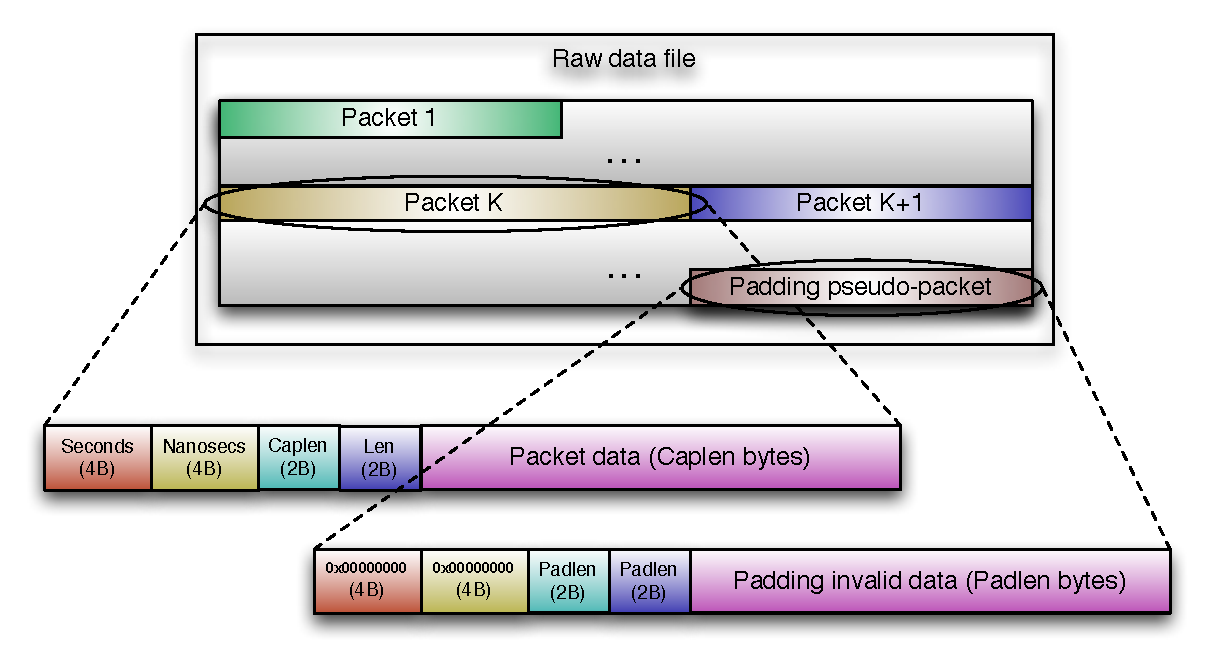
\includegraphics[angle=0,width=\textwidth]{figs/buff_raw2.pdf}
		\caption{Raw file format}
		\label{fig:rawformat}
	\end{center}
\end{figure}


The end of the file is denoted by the appearance of a pseudo packet showing the amount of padding bytes added at the end of the file (in order to generate files of the same size).
The padding pseudo-packet has a similar header than any other packet in the file with the difference that both the "Seconds" and the "Nanoseconds" fields are set to zeros.
Once the padding pseudo-packet has been located, the padding size can be read from any of the "Len" or "Caplen" fields. Note that the padding length could be zero.

\subsection{Example code}

The file \textit{raw2pcap.c} in the \textit{samples/raw2pcap} folder is an example of a program that reads a raw file and generates a new pcap file with the contents of the first one.





\nocite{*}
\bibliographystyle{unsrt}
\bibliography{hpcap_dpro10g}

\end{document}
